%%%%%%%%%%%%%%%%%%%%%%%%%%%%%%%%%%%%%%%%%%%%%%%%%%%%%%%%%%%%
%%  This Beamer template was created by Cameron Bracken.
%%  Anyone can freely use or modify it for any purpose
%%  without attribution.
%%
%%  Last Modified: January 9, 2009
%%

\documentclass[xcolor=x11names,compress]{beamer}

%% General document %%%%%%%%%%%%%%%%%%%%%%%%%%%%%%%%%%
\usepackage{graphicx}
\usepackage{tikz}
\usepackage{amsmath}
\usepackage{amssymb}
\usepackage{amsthm}
\usepackage{acronym}
\usepackage{chngpage}
\usepackage{bbm}
\usepackage{tikz, overpic}
\usepackage{empheq} % autoloads mathtols and amsmath
\usepackage{multirow}%tex
\usepackage{pifont}
\usepackage{rotating}
\usepackage{subcaption}
\usepackage{pgfplots}
\usepackage{adjustbox}

\newcommand{\bsum}[2]{\sum_{#1}^{#2}}
\newcommand{\bint}[2]{\int_{#1}^{#2}}
\newcommand{\E}[1]{\mathrm{E}(#1)}
\newcommand{\Var}[1]{\mathrm{Var}(#1)}
\newcommand{\Cov}[1]{\mathrm{Cov}(#1)}
\newcommand\given[1][]{\:#1\vert\:}
\newcommand{\for}{\;\text{for}\;}
\newcommand{\aand}{\;\text{and}\;}
\def\MLine#1{\par\hspace*{-\leftmargin}\parbox{\textwidth}{\[#1\]}}

\newcommand{\cmark}{\ding{51}}%
\newcommand{\xmark}{\ding{55}}%

%%%%%%%%%%%%%%%%%%%%%%%%%%%%%%%%%%%%%%%%%%%%%%%%%%%%%%


%% Beamer Layout %%%%%%%%%%%%%%%%%%%%%%%%%%%%%%%%%%
\useoutertheme[subsection=false,shadow]{miniframes}
\useinnertheme{default}
\usefonttheme{serif}
\usepackage{palatino}


\usetikzlibrary{bayesnet}


\setbeamerfont{title like}{shape=\scshape}
\setbeamerfont{frametitle}{shape=\scshape}

\setbeamercolor*{lower separation line head}{bg=DeepSkyBlue4} 
\setbeamercolor*{normal text}{fg=black,bg=white} 
\setbeamercolor*{alerted text}{fg=red} 
\setbeamercolor*{example text}{fg=black} 
\setbeamercolor*{structure}{fg=black} 
 
\setbeamercolor*{palette tertiary}{fg=black,bg=black!10} 
\setbeamercolor*{palette quaternary}{fg=black,bg=black!10} 

\addtobeamertemplate{navigation symbols}{}{%
    \usebeamerfont{footline}%
    \usebeamercolor[fg]{footline}%
    \hspace{1em}%
    \insertframenumber/\inserttotalframenumber
}


\renewcommand{\(}{\begin{columns}}
\renewcommand{\)}{\end{columns}}
\newcommand{\<}[1]{\begin{column}{#1}}
\renewcommand{\>}{\end{column}}
%%%%%%%%%%%%%%%%%%%%%%%%%%%%%%%%%%%%%%%%%%%%%%%%%%




\begin{document}


%%%%%%%%%%%%%%%%%%%%%%%%%%%%%%%%%%%%%%%%%%%%%%%%%%%%%%
%%%%%%%%%%%%%%%%%%%%%%%%%%%%%%%%%%%%%%%%%%%%%%%%%%%%%%
\section{\scshape Introduction}
\subsection{Intro}
\begin{frame}
\title{State-Aware TrueSkill For Tennis Prediction}
\author{
	Hin Hong TAM (Ryan)\\
	{\it Imperial College London}\\
}
\date{
	\vspace{1cm}
	\today
}
\titlepage
\end{frame}

\subsection{Goals}
\begin{frame}{Goals}
	\begin{itemize}[<+->]
		\item Comprehensive Overview Of TrueSkill
		\item Use TrueSkill To Model Tennis
		\item Forumulate And Experiment \textit{State-Aware} TrueSkill
		\item Use State-Aware TrueSkill To Model Tennis
	\end{itemize}
\end{frame}

%%%%%%%%%%%%%%%%%%%%%%%%%%%%%%%%%%%%%%%%%%%%%%%%%%%%%%
%%%%%%%%%%%%%%%%%%%%%%%%%%%%%%%%%%%%%%%%%%%%%%%%%%%%%%
\section{\scshape TrueSkill}
\subsection{Formulation}
\begin{frame}{Formulation Of TrueSkill}
	\begin{columns}
		\begin{column}{0.6\textwidth}
			\begin{itemize}[<+->]
				\item Uses Factor Graph
				\item \MLine{Pr(\vec{s}, \vec{r}) = {Pr(\vec{r}\given \vec{s})Pr(\vec{s})}}
				\item Factorising Priors
				\MLine{Pr(\vec{s}) \triangleq \prod_{i=1}^{n} Pr(s_i)}
				\item Factorising Likelihood
				\MLine{Pr(\vec{r} \given s_1, s_2 ) \triangleq Pr(p_1 \given s_1) Pr (p_2\given s_2) Pr(d \given p_1,p_2) Pr(\vec{r}\given d)}
			\end{itemize}
		\end{column}
		\begin{column}{0.4\textwidth}
			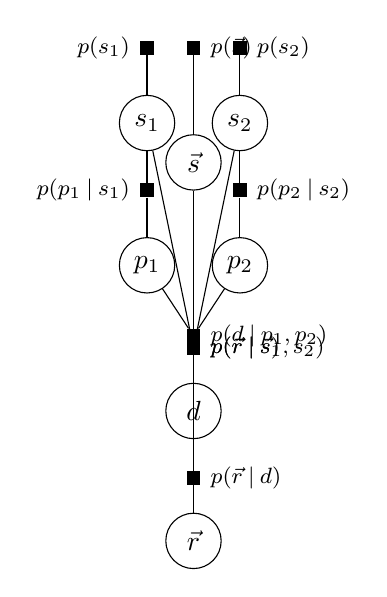
\begin{tikzpicture}
				\onslide<2> \factor {fs} {right:$p(\vec{s})$} {} {};
				\onslide<2> \node[latent, below=of fs] (s) {$\vec{s}$};
				\onslide<3-> \factor[left=of fs] {fs1} {left:$p(s_1)$} {} {};
				\onslide<3-> \factor[right=of fs] {fs2} {right:$p(s_2)$} {} {};
				\onslide<3-> \node[latent, below=of fs1, yshift=0.5cm] (s1) {$s_1$};
				\onslide<3-> \node[latent, below=of fs2, yshift=0.5cm] (s2) {$s_2$};
				
				\onslide<4-> \factor[below=of s1]{fsp1} {left:$p(p_1\given s_1)$} {} {};
				\onslide<4-> \factor[below=of s2]{fsp2} {right:$p(p_2\given s_2)$} {} {};
				\onslide<4-> \node[latent, below=of fsp1, yshift=0.5cm] (p1) {$p_1$};
				\onslide<4-> \node[latent, below=of fsp2, yshift=0.5cm] (p2) {$p_2$};
				
				
				\onslide<2> \factor[below=of s, yshift=-1.5cm] {frs} {right:$p(\vec{r}\given \vec{s})$} {} {};
				\onslide<3> \factor[below=of s, yshift=-1.5cm] {frs12} {right:$p(\vec{r}\given s_1,s_2)$} {} {};
				\onslide<2->\node[latent, below=of frs, yshift=-1cm] (r) {$\vec{r}$};
				\onslide<4-> \factor[above=of r, yshift=1.75cm] {fd}{right:$p(d \given p_1, p_2)$} {} {};
				\onslide<4-> \node[latent, below=of fd,yshift=0.5cm] (d) {$d$};		
				\onslide<4-> \factor[below=of d] {frd}{right:$p(\vec{r} \given d)$} {} {};
				

				
				\onslide<2>\factoredge[-]{fs}{s}{frs};
				\onslide<2-3>\factoredge[-]{}{frs}{r};
				\onslide<3>\factoredge[-]{fs1}{s1}{frs};
				\onslide<3>\factoredge[-]{fs2}{s2}{frs};
				
				\onslide<4> \factoredge[-]{fs1}{s1}{fsp1};
				\onslide<4> \factoredge[-]{fs2}{s2}{fsp2};
				\onslide<4> \factoredge[-]{fsp1}{p1}{fd};
				\onslide<4> \factoredge[-]{fsp2}{p2}{fd};
				\onslide<4> \factoredge[-]{fd}{d}{frd};
				\onslide<4> \factoredge[-]{}{frd}{r};
				
				

			\end{tikzpicture}
		\end{column}
	\end{columns}
\end{frame}

\begin{frame}{Specification Of Factors In TrueSkill}
	\begin{columns}
		\begin{column}{0.6\textwidth}
			\begin{itemize}[<+->]
				\item Gaussian Skill Priors 
				\vspace{-0.25cm}
				$$p(s_i) = \mathcal{N}(s_i \given \mu_i, \sigma_i^2 + \tau^2)$$
				\item Skill-Performance Factors
				\vspace{-0.25cm}
				$$p(p_i \given s_i) = \mathcal{N}(p_i \given s_i, \beta^2)$$
				\item Performance-Differencing Factor
				\vspace{-0.25cm}
				$$p(d \given p_1, p_2) = \mathbb{I}(d=p_1-p_2)$$ 
				\item Outcome-Truncation Factor
				\vspace{-0.25cm}
				$$p(r \given d) = \mathbb{I}(d > 0) \text{ if player 1 won}$$
				\vspace{-0.75cm}
				$$p(r \given d) = \mathbb{I}(d < 0) \text{ if player 2 won}$$
			\end{itemize}
		\end{column}
		\begin{column}{0.4\textwidth}
			\begin{tikzpicture}
\factor[left=of fs] {fs1} {left:$p(s_1)$} {} {};
\factor[right=of fs] {fs2} {right:$p(s_2)$} {} {};
\node[latent, below=of fs1, yshift=0.5cm] (s1) {$s_1$};
\node[latent, below=of fs2, yshift=0.5cm] (s2) {$s_2$};

\factor[below=of s1]{fsp1} {left:$p(p_1\given s_1)$} {} {};
\factor[below=of s2]{fsp2} {right:$p(p_2\given s_2)$} {} {};
\node[latent, below=of fsp1, yshift=0.5cm] (p1) {$p_1$};
\node[latent, below=of fsp2, yshift=0.5cm] (p2) {$p_2$};

\node[latent, below=of frs, yshift=-1cm] (r) {$\vec{r}$};
\factor[above=of r, yshift=1.75cm] {fd}{right:$p(d \given p_1, p_2)$} {} {};
\node[latent, below=of fd,yshift=0.5cm] (d) {$d$};		
\factor[below=of d] {frd}{right:$p(\vec{r} \given d)$} {} {};

\factoredge[-]{fs1}{s1}{fsp1};
\factoredge[-]{fs2}{s2}{fsp2};
\factoredge[-]{fsp1}{p1}{fd};
\factoredge[-]{fsp2}{p2}{fd};
\factoredge[-]{fd}{d}{frd};
\factoredge[-]{}{frd}{r};
				
			\end{tikzpicture}
		\end{column}
	\end{columns}
\end{frame}


\subsection{Factor Graph}
\begin{frame}{Factor Graph Example}
	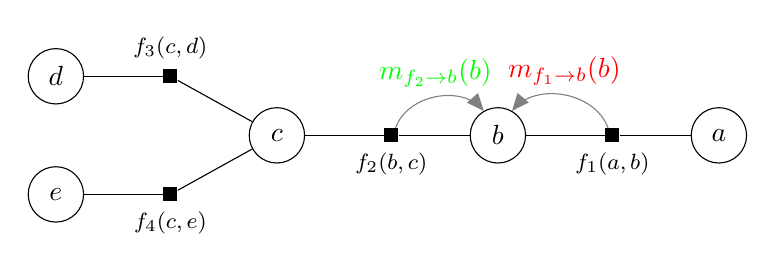
\begin{tikzpicture}
		\node[latent] (a) {$a$};
		\factor[left=of a, xshift=-0.5cm] {fab} {below:$f_1(a,b)$} {} {};
		\node[latent, left=of fab] (b) {$b$};
		\factor[left=of b, xshift=-0.5cm] {fbc} {below:$f_2(b,c)$} {} {};
		\node[latent, left=of fbc] (c) {$c$};
		\factor[left=of c, yshift=0.75cm, xshift=-0.5cm] {fcd} {above:$f_3(c,d)$} {} {};
		\factor[left=of c, yshift=-0.75cm, xshift=-0.5cm] {fce} {below:$f_4(c,e)$} {} {};
		\node[latent, left=of fcd] (d) {$d$};
		\node[latent, left=of fce] (e) {$e$};
		
		\factoredge[-] {a} {fab} {b};
		\factoredge[-] {b} {fbc} {c};
		\factoredge[-] {c} {fcd} {d};
		\factoredge[-] {c} {fce} {e};
		
		\onslide<3> \cgate{left}{(a)(fab)(fab-caption)}{};
		\onslide<3> \cgate{right}{(fbc)(fbc-caption)(c)(fcd)(fcd-caption)(fce)(fce-caption)(d)(e)}{};
		\onslide<4> \draw [gray,->] (fab) edge [bend right=60] node [red, above] {$m_{f_1\rightarrow b} (b) $} (b);
		\onslide<4> \draw [gray,->] (fbc) edge [bend left=60] node [green, above] {$m_{f_2\rightarrow b}(b)$} (b);
		
	\end{tikzpicture}
	\begin{itemize}[<+->]
		\item[]<2-> \MLine{ p(b) = \bsum{a}{} \bsum{c}{}\bsum{d}{}\bsum{e}{}
		f_1(a,b)f_2(b,c)f_3(c,d)f_4(c,e)}
		\item[]<3-> \MLine{ \implies p(b) = \only<4>{\color{red}}{\bsum{a}{} f_1(a,b)} \color{black}{\times} \only<4>{\color{green}}{[\bsum{c}{}\bsum{d}{}\bsum{e}{} f_2(b,c)f_3(c,d)f_4(c,e)]}}
		
	\end{itemize}		
\end{frame}



\begin{frame}{Factor Graph}
	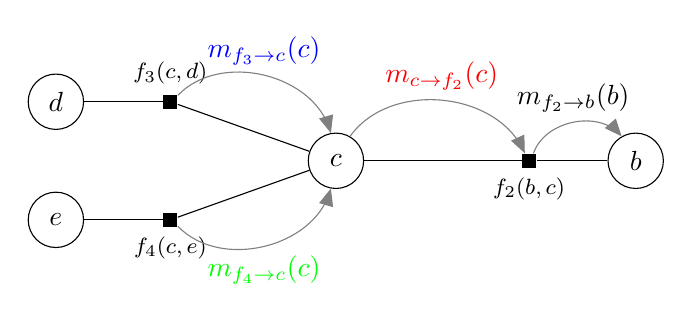
\begin{tikzpicture}
		\node[latent] (b) {$b$};
		\factor[left=of b, xshift=-0.5cm] {fbc} {below:$f_2(b,c)$} {} {};
		\node[latent, left=of fbc, xshift=-1cm] (c) {$c$};
		\factor[left=of c, yshift=0.75cm, xshift=-1.25cm] {fcd} {above:$f_3(c,d)$} {} {};
		\factor[left=of c, yshift=-0.75cm, xshift=-1.25cm] {fce} {below:$f_4(c,e)$} {} {};
		\node[latent, left=of fcd] (d) {$d$};
		\node[latent, left=of fce] (e) {$e$};
		
		\factoredge[-] {b} {fbc} {c};
		\factoredge[-] {c} {fcd} {d};
		\factoredge[-] {c} {fce} {e};
		

		\draw [gray,->] (fbc) edge [bend left=60] node [black, above] {$m_{f_2\rightarrow b}(b)$} (b);
		\onslide<3-4> \draw [gray,->] (c) edge [bend left=60] node [red, above] {$m_{c\rightarrow f_2}(c)$} (fbc);
		\onslide<5> \draw [gray,->] (fcd) edge [bend left=60] node [blue, above] {$m_{f_3\rightarrow c}(c)$} (c);
		\onslide<5> \draw [gray,->] (fce) edge [bend right=60] node [green, below] {$m_{f_4\rightarrow c}(c)$} (c);
		
		
	\end{tikzpicture}
	\begin{itemize}[<+->]
		\item[] \MLine{ m_{f_2\rightarrow b}(b) = \bsum{c}{}\bsum{d}{}\bsum{e}{} f_2(b,c)f_3(c,d)f_4(c,e)}
		\item[]<2-> \MLine{
			 \implies m_{f_2\rightarrow b}(b) = \bsum{c}{} [f_2(b,c) 
			 \only<3-4>{\color{red}}
			 \only<2-3>{[\bsum{d}{}\bsum{e}{} f_3(c,d)f_4(c,e)}
			 \only<4>{[\bsum{d}{}f_3(c,d)][\bsum{e}{} f_4(c,e)]}
			 \only<5>{\color{blue}[\bsum{d}{}f_3(c,d)]\color{green}[\bsum{e}{} f_4(c,e)]}
			 \color{black}]]
		}		
		
		
		
		
		

	\end{itemize}
\end{frame}

\begin{frame}{Sum-Product Algorithm}
	\begin{itemize}[<+->]
		\item<1-> Variable Node To Factor Node 
		\item[]<1-> \MLine{m_{x_m \rightarrow f_s} (x_m) = 
		\only<5>{\color{red}}\prod_{l\in ne(x_m) \setminus f_s} \left(m_{f_l \rightarrow x_m} (x_m)\right)}\color{black}
		\item<2-> Factor Node To Variable Node 
		\item[]<2-> \vspace{-0.25cm} \MLine{m_{f_s \rightarrow x}(x) = \bsum{x_1}{} \cdots \bsum{x_M}{} \left( f_s (x,x_1,\dots,x_M) \prod_{i\in ne(f_s)\setminus x} \left(m_{x_i \rightarrow f_s}(x_i)\right)\right)}
		
		\item<3-> Marginal
		\MLine{p(x) = \prod_{f_i \in ne(x)} m_{f_i \rightarrow x} (x)}
		\onslide<4-5>{\MLine{ \implies p(x) = m_{{f} \rightarrow x} (x) \only<5>{\color{red}}\prod_{f_i \in ne(x) \setminus {f}} m_{f_i \rightarrow x} (x) \color{black} \;\;\;\forall\; {f} \in ne(x)}}

	\end{itemize}
\end{frame}



\pgfmathdeclarefunction{gauss}{2}{%
  \pgfmathparse{1/(#2*sqrt(2*pi))*exp(-((x
  -#1)^2)/(2*#2^2))}%
}
\pgfmathdeclarefunction{line}{1}{%
  \pgfmathparse{#1}%
}



\subsection{Result}
\begin{frame}{Results On Seperate Test Set}

\begin{table}[H] \centering 

\begin{tabular}{@{\extracolsep{5pt}} cccc} 
\\[-1.8ex]\hline 
\hline \\[-1.8ex] 
Data  & Selection & Brier  & Error  \\ 
Granularity & Based On & Score & Rate \\
\hline \\[-1.8ex] 
Match & Brier & $0.199784$ & $0.312693$ \\ 
Match & Error & $0.202965$ & $0.319917$ \\ 
Point & Brier & $0.249268$ & $0.477656$ \\ 
Point & Error & $0.249284$ & $0.477803$ \\ 
\hline \\[-1.8ex] 
\end{tabular} 
  \caption{Performance On A Separate Test Set Of Na\"{i}ve Models} 
\end{table} 

\end{frame}







\section{\scshape State-Aware TrueSkill}
\subsection{Formulation}

\begin{frame}{Factor Graph Representation}
\begin{adjustbox}{max totalsize={1\textwidth}{.9\textheight},center}
    \begin{tikzpicture}[scale=0.33]
        % left
        \factor[]{s-factor1}{left:$\mathcal{N}(s_1 \given \mu_1, \sigma_1^2+\tau^2)$}{}{};
        \node[latent, below=of s-factor1, yshift=0.5cm] (s1) {$s_1$};
        \factor[below=of s1, yshift=-0.5cm]{sp-factor1}{left:$\mathcal{N}(p_1 \given s_1 +, \beta^2)$} {}{};
        \node[latent, below=of sp-factor1, yshift=0.5cm] (p1) {$p_1$};
        \factor[below=of p1, xshift=-1.3cm, yshift=-0.1cm] {pt-factor1} {left:$\mathbbm{I}(t_1=p_1+ \eta a_1)$}{}{};
        \node[latent, below=of pt-factor1, yshift=0.5cm] (t1) {$t_1$};
        
        % left adj 
        \factor[left=of sp-factor1, xshift=-2cm] {a-factor1}{left:$\mathcal{N}(a_1 \given \mu_{a_1}, \sigma^2_{a_1} +\tau^2_a)$}{}{};
        \node[latent, below=of a-factor1, yshift=0.5cm](a1){$a_1$};
        \edge[-]{pt-factor1}{a1}
        \edge[-]{a-factor1}{a1}
        
        % left-connections
        \edge[-]{s-factor1}{s1}
        \edge[-]{s1}{sp-factor1}
        \edge[-]{sp-factor1}{p1}
        \edge[-]{p1}{pt-factor1}
        \edge[-]{pt-factor1}{t1}
        
        
        % right
        \factor[right=of s-factor1,xshift=3cm]{s-factor2}{right:$\mathcal{N}(s_2 \given \mu_2, \sigma_2^2+\tau^2)$}{}{};
        \node[latent, below=of s-factor2, yshift=0.5cm] (s2) {$s_2$};
        \factor[below=of s2, yshift=-0.5cm]{sp-factor2}{right:$\mathcal{N}(p_2 \given s_2, \beta^2)$} {}{};
        \node[latent, below=of sp-factor2, yshift=0.5cm] (p2) {$p_2$};
        \factor[below=of p2, , xshift=1.3cm, yshift=-0.1cm] {pt-factor2} {right:$\mathbbm{I}(t_2=p_2+ \eta a_2)$}{}{};
        \node[latent, below=of pt-factor2, yshift=0.5cm] (t2) {$t_2$};
        
        % right-connections
        \edge[-]{s-factor2}{s2}
        \edge[-]{s2}{sp-factor2}
        \edge[-]{sp-factor2}{p2}
        \edge[-]{p2}{pt-factor2}
        \edge[-]{pt-factor2}{t2}
        
        % right adj 
        \factor[right=of sp-factor2, xshift=2cm] {a-factor2}{right:$\mathcal{N}(a_2 \given \mu_{a_2}, \sigma^2_{a_2} +\tau^2_a)$}{}{};
        \node[latent, below=of a-factor2, yshift=0.5cm](a2){$a_2$};
        \edge[-]{pt-factor2}{a2}
        \edge[-]{a-factor2}{a2}
        
        
        
        % middle 
        \factor[below=of t1, xshift=3.2cm, yshift=-0.5cm] {td-factor} {left:$\mathbbm{I}(d=t_1-t_2)$}{}{};
        \node[latent, below=of td-factor](d) {$d$};
        \factor[below=of d] {d-factor} {left:$\mathbbm{I}(d>\epsilon)$}{}{};
        
        % middle-connections
        \edge[-]{t1}{td-factor}
        \edge[-]{t2}{td-factor}
        \edge[-]{td-factor}{d}
        \edge[-]{d}{d-factor}
    
        
        \end{tikzpicture}
\end{adjustbox}
\end{frame}



\subsection{Results}
\begin{frame}{Point Level Results On ATP Dataset}

\begin{itemize}[<+->]
	\item Selection Of $\beta$ : $21 \rightarrow 10$
	\item Brier Score : $0.249268 \rightarrow 0.225575$
	\item Error Rate: $0.477656 \rightarrow 0.349461$ 			
\end{itemize}



\end{frame}


\section{\scshape Conclusion}
\begin{frame}{Future Work}

\begin{itemize}[<+->]
	\item Extending The Model To Cover Multiplayer Games
	\item Elegantly Deal With Continuous Features
	\item Include Other Features Of Tennis
	\item Dissociation Of Features
\end{itemize}
\end{frame}






\end{document}
